\documentclass[a4paper, 11pt]{article}
\usepackage{comment} % enables the use of multi-line comments (\ifx \fi) 
\usepackage{lipsum} %This package just generates Lorem Ipsum filler text. 
\usepackage{fullpage} % changes the margin
\usepackage[a4paper, total={7in, 10in}]{geometry}
\usepackage[fleqn]{amsmath}
\usepackage{amssymb,amsthm}  % assumes amsmath package installed
\newtheorem{theorem}{Theorem}
\newtheorem{corollary}{Corollary}
\usepackage{graphicx}
\usepackage{caption}
\usepackage{bm}

% \usepackage[pdftex]{graphicx}
\usepackage{tikz}
\usetikzlibrary{arrows}
\usepackage{verbatim}
\usepackage[numbered]{mcode}
\usepackage{float}
\usepackage{tikz}
    \usetikzlibrary{shapes,arrows}
    \usetikzlibrary{arrows,calc,positioning}

    \tikzset{
        block/.style = {draw, rectangle,
            minimum height=1cm,
            minimum width=1.5cm},
        input/.style = {coordinate,node distance=1cm},
        output/.style = {coordinate,node distance=4cm},
        arrow/.style={draw, -latex,node distance=2cm},
        pinstyle/.style = {pin edge={latex-, black,node distance=2cm}},
        sum/.style = {draw, circle, node distance=1cm},
    }
\usepackage{xcolor}
\usepackage{mdframed}
\usepackage[shortlabels]{enumitem}
\usepackage{indentfirst}
\usepackage{hyperref}
\usepackage{CJKutf8}
    
\renewcommand{\thesubsection}{\thesection.\alph{subsection}}

\newenvironment{problem}[2][Q]
    { \begin{mdframed}[backgroundcolor=gray!20] \textbf{#1 #2} \\}
    {  \end{mdframed}}

% Define solution environment
\newenvironment{solution}
    {\textit{Solution:}}
    {}

\renewcommand{\qed}{\quad\qedsymbol}
%%%%%%%%%%%%%%%%%%%%%%%%%%%%%%%%%%%%%%%%%%%%%%%%%%%%%%%%%%%%%%%%%%%%%%%%%%%%%%%%%%%%%%%%%%%%%%%%%%%%%%%%%%%%%%%%%%%%%%%%%%%%%%%%%%%%%%%%
\begin{document}
\begin{CJK}{UTF8}{gbsn}
%Header-Make sure you update this information!!!!
\noindent
%%%%%%%%%%%%%%%%%%%%%%%%%%%%%%%%%%%%%%%%%%%%%%%%%%%%%%%%%%%%%%%%%%%%%%%%%%%%%%%%%%%%%%%%%%%%%%%%%%%%%%%%%%%%%%%%%%%%%%%%%%%%%%%%%%%%%%%%
\large\textbf{课程: 人工智能} \hfill \textbf{作业 6}   \\
北航软件学院 \\
\normalsize 学期: 2023，春季\hfill 提交截止时间:  2023年6月30日, 11：59 PM \\
\noindent\rule{7in}{2.8pt}
\textbf{提醒注意:}
\begin{itemize}
\item 本次作业发布于2023年6月2日，截止于2023年6月30日。
\item 作业一分为三部分：问答题、实训题、以及实训题报告
\begin{itemize}
    \item 问答题答案可以手写并扫描，或者用latex（或word）手打，最终以QA.pdf文件命名。
    \item 实训题按照项目共享链接内要求和基础代码进行作答。
    \item 报告部分同样可以手写或者手打，以Report.pdf文件命名。
    \item 作业提交格式：$<student ID>$\_$<name>$\_A6.zip。比如1921102\_田嘉怡\_A6.zip
    \item 提交的zip文件要求（仅）包括：
    \begin{itemize}
        \item 实训题文件：包括 main.py（或main.ipynb）。
        \item 问答题答案：QA.pdf
        \item 报告：Report.pdf。需要包含实训题2.3、2.6部分的运行截图。
    \end{itemize}
    
\end{itemize}
\item 作业压缩包需要在spoc平台上提交。
\item 每迟交1天（不满1天按1天计算），本次作业扣除10\%分数。
\item 不按作业要求和格式提交，视情况扣分。不得抄袭。
\end{itemize}

\noindent\rule{7in}{1pt}
\textbf{第一部分：问答题（共6分）}
% %%%%%%%%%%%%%%%%%%%%%%%%%%%%%%%%%%%%%%%%%%%%%%%%%%%%%%%%%%%%%%%%%%%%%%%%%%%%%%%%%%%%%%%%%%%%%%%%%%%%%%%%%%%%%%%%%%%%%%%%%%%%%%%%%%%%%%%%
% % Problem 1
% %%%%%%%%%%%%%%%%%%%%%%%%%%%%%%%%%%%%%%%%%%%%%%%%%%%%%%%%%%%%%%%%%%%%%%%%%%%%%%%%%%%%%%%%%%%%%%%%%%%%%%%%%%%%%%%%%%%%%%%%%%%%%%%%%%%%%%%%
% \begin{problem}{1}
% % (本题不好回答)以机器为载体来模拟人类智能的某一方面，可以通过以符号主义为核心的逻辑推理、以问题求解为核心的探寻搜索、以数据驱动为核心的机器学习、以行为主义为核心的强化学习、以博弈对抗为核心的决策智能等方法来实现。请比较上述人工智能不同方法的优劣。
% \end{problem}

%%%%%%%%%%%%%%%%%%%%%%%%%%%%%%%%%%%%%%%%%%%%%%%%%%%%%%%%%%%%%%%%%%%%%%%%%%%%%%%%%%%%%%%%%%%%%%%%%%%%%%%%%%%%%%%%%%%%%%%%%%%%%%%%%%%%%%%%
% Problem 1
%%%%%%%%%%%%%%%%%%%%%%%%%%%%%%%%%%%%%%%%%%%%%%%%%%%%%%%%%%%%%%%%%%%%%%%%%%%%%%%%%%%%%%%%%%%%%%%%%%%%%%%%%%%%%%%%%%%%%%%%%%%%%%%%%%%%%%%%


\begin{problem}{1（1分）}
将机器人寻路问题简化为图1的2*2的网格，假设有位于$s_1$位置的机器人拟从$s_1$这一初始位置向$s_4$这一目标位置移动。机器人每次只能向上或者向右移动一个方格，到达目标位置$s_4$则会获得奖励且游戏终止，机器人在移动过程中如果越出方格($s_d$)则会被惩罚且被损坏、并且游戏终止。奖励值定义如下：当$S_{t+1}=s_4$时奖励值为1，当$S_{t+1}=s_d$时惩罚值为-1，其他情况下奖励值为0。若折扣因子γ=0.99，智能体在$s_1$、$s_2$、$s_3$的策略都初始化为上，终止状态$s_4$、$s_d$的价值函数定义为0，试通过联立贝尔曼方程给出状态$s_1$、$s_2$、$s_3$的价值函数。
\begin{figure}[H]
    \centering
    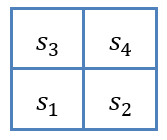
\includegraphics[width=0.15\textwidth]{P1.PNG}
    \caption{2*2的机器人寻路问题}
    \label{fig:my_label}
\end{figure}
\end{problem}


%%%%%%%%%%%%%%%%%%%%%%%%%%%%%%%%%%%%%%%%%%%%%%%%%%%%%%%%%%%%%%%%%%%%%%%%%
% Problem 2
%%%%%%%%%%%%%%%%%%%%%%%%%%%%%%%%%%%%%%%%%%%%%%%%%%%%%%%%%%%%%%%%%%%%%%%%%%%%%%%%%%%%%%%%%%%%%%%%%%%%%%%%%%%%%%%%%%%%%%%%%%%%%%%%%%%%%%%%
\begin{problem}{2（2分）}
在题1中，若每个状态的价值函数都初始化为0，智能体在$s_1$、$s_2$、$s_3$的策略都初始化为上，试优化智能体在状态$s_3$的策略。（提示：使用策略优化定理）
\end{problem}

% \vspace{4em}
\newpage
%%%%%%%%%%%%%%%%%%%%%%%%%%%%%%%%%%%%%%%%%%%%%%%%%%%%%%%%%%%%%%%%%%%%%%%%%
% Problem 3
%%%%%%%%%%%%%%%%%%%%%%%%%%%%%%%%%%%%%%%%%%%%%%%%%%%%%%%%%%%%%%%%%%%%%%%%%%%%%%%%%%%%%%%%%%%%%%%%%%%%%%%%%%%%%%%%%%%%%%%%%%%%%%%%%%%%%%%%


\begin{problem}{3（3分）}
在题1中，若图2表示算法的初始状态，其中a/b表示对应状态的动作-价值函数的取值，斜线左侧的a表示$q_{\pi}$(s,上)，斜线右侧的b表示$q_{\pi}$(s,右)。若α=0.5，试给出Q Learning 算法中的Q学习算法的一个片段的执行过程，并给出执行完该片段后每个状态的策略。
\begin{figure}[H]
    \centering
    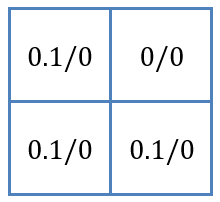
\includegraphics[width=0.15\textwidth]{P2.PNG}
    \caption{Q学习算法的初始状态}
    \label{fig:my_label} 
\end{figure}
\end{problem}



%%%%%%%%%%%%%%%%%%%%%%%%%%%%%%%%%%%%%%%%%%%%%%%%%%%%%%%%%%%%%%%%%%%%%%%%%
% Problem 4
%%%%%%%%%%%%%%%%%%%%%%%%%%%%%%%%%%%%%%%%%%%%%%%%%%%%%%%%%%%%%%%%%%%%%%%%%%%%%%%%%%%%%%%%%%%%%%%%%%%%%%%%%%%%%%%%%%%%%%%%%%%%%%%%%%%%%%%%



\noindent\rule{7in}{1pt}
\textbf{第二部分：实训题（共6分）}
\\ \\
\textbf{实训题要求:}
\begin{itemize}
    \item 本次作业包括1个实训题，作业要求以及基础代码以Aistudio项目的形式发布。
    \item 发布项目链接有效期3天，请在作业发布3天内fork这个项目，生成``我的项目''，并在自己fork的项目下进行作答，生成答案后按要求保存提交。
\end{itemize}

%%%%%%%%%%%%%%%%%%%%%%%%%%%%%%%%%%%%%%%%%%%%%%%%%%%%%%%%%%%%%%%%%%%%%%%%%
% Problem 1
%%%%%%%%%%%%%%%%%%%%%%%%%%%%%%%%%%%%%%%%%%%%%%%%%%%%%%%%%%%%%%%%%%%%%%%%%%%%%%%%%%%%%%%%%%%%%%%%%%%%%%%%%%%%%%%%%%%%%%%%%%%%%%%%%%%%%%%%

\begin{problem}{1 机器人自走迷宫-强化学习}

在本作业中，您首先需要阅读开发代码中需要用到的基础知识，包括我们代码中会用到的Maze迷宫类、QRobot类、Runner类。再之后您有一些任务需要完成，我们将根据任务完成的情况来给予您的分数。  
作业分为两各部分
\begin{itemize}
    \item 第一部分：实现2.3部分的搜索算法，您可任选深度优先搜索算法、最佳优先搜索（A*)算法实现其中一种。
    \item 第二部分：实现2.6部分的Deep QLearning (DQN)算法，公共部分可复用，您只需要重写Robot类中的train\_update()、 test\_update()方法即可，可参考QRobot类中的train\_update()和test\_update() 接口实现的Q Learing算法。
\end{itemize}
实验介绍详情和参考基础代码请参见Aistudio中的共享项目\href{https://aistudio.baidu.com/studio/project/partial/verify/5522785/61f8ecf180ac43398f90e36520c41018}{“人工智能作业六-机器人自走迷宫”}。
\end{problem}

\noindent\rule{7in}{1pt}
\textbf{第三部分：实训题实验报告（共3分）}
\begin{itemize}
    \item 请按照实验报告模板完成实验报告。
    \item 实验报告模板是通用模板，可根据每个作业要求的差别，自由进行微调。
\end{itemize}

\end{CJK}
\end{document}